\begin{frame}[fragile]{Tutorial: n-site states with MPS}

\begin{columns}

\begin{column}{5.5cm}

\begin{onlyenv}<1->
%% Definition of $\psi_\theta$, not enough space to include in slide.
%% $\psi_\theta$ = apply(U($\theta$, i; nlayers=nlayers), $\psi_0$;
%%            maxdim=maxdim, cutoff=cutoff)
\begin{lstlisting}[language=JuliaLocal, style=julia, mathescape, basicstyle=\small]
$\psi_0$ = MPS(i, "Z+")
nlayers = 6
function E($\theta$)
  $\psi_\theta$ = apply(U($\theta$, i; nlayers), $\psi_0$)
  return inner($\psi_\theta$', H, $\psi_\theta$)
end

$\theta_0$ = zeros(nlayers * n)
$\theta$ = minimize(E, $\partial$E, $\theta_0$;
      nsteps=20, $\gamma$=0.1)
\end{lstlisting}
\end{onlyenv}

\begin{onlyenv}<3->
\begin{lstlisting}[language=JuliaLocal, style=julia, mathescape, basicstyle=\small]
maxlinkdim($\psi_0$)
maxlinkdim($\psi_\theta$)
E($\theta_0$), norm($\partial$E($\theta_0$))
E($\theta$), norm($\partial$E($\theta$))
\end{lstlisting}
\end{onlyenv}

\end{column}

\begin{column}{4.5cm}

\begin{onlyenv}<1-1>
|0$\rangle$ = |Z+Z+…Z+$\rangle$ \\
~\\
Minimize over $\theta$: \\
|$\theta\rangle$ = U($\theta$)|0$\rangle$ \\
E($\theta$) = $\langle\theta$|H|$\theta\rangle$ \\
~\\
~\\
~\\
~\\
~\\
\end{onlyenv}

\begin{onlyenv}<2->
\vspace*{0.0cm}
\begin{center}
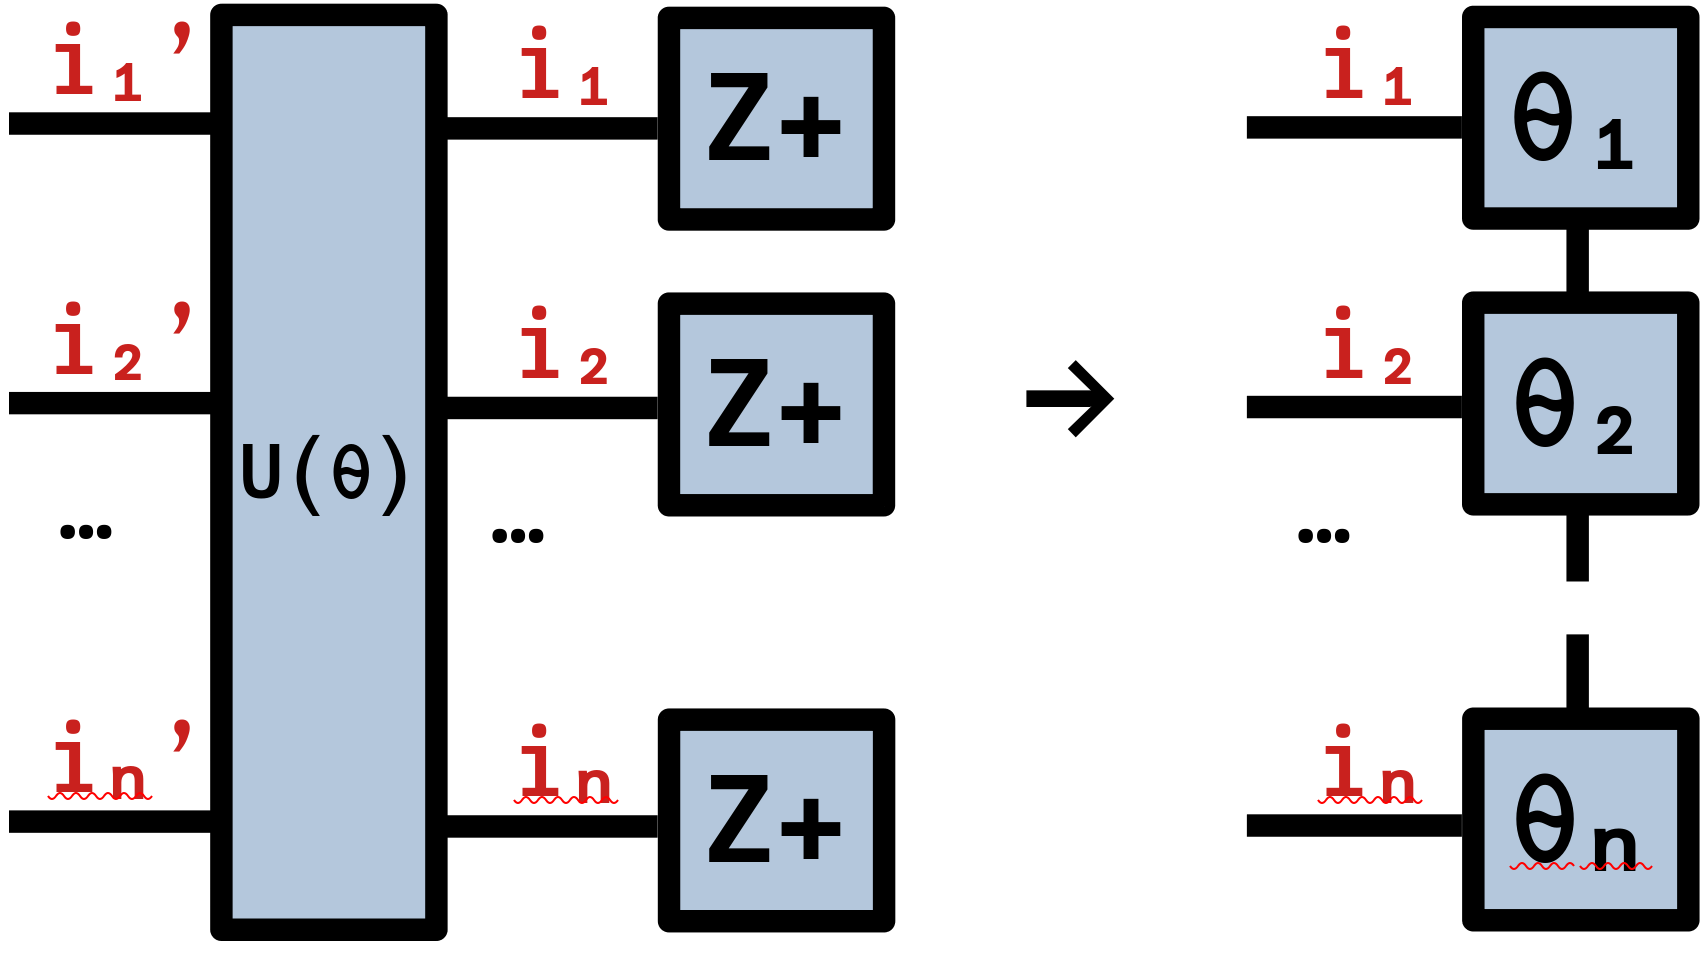
\includegraphics[width=\textwidth]{
  slides/assets/U_Zpn.png
}
\end{center}
\vspace*{0.0cm}
\end{onlyenv}

\begin{onlyenv}<3-3>
1 (product state) \\
2 (entangled state) \\
(-29, 5.773335) \\
(-31.017062, 0.000759)
\end{onlyenv}

\begin{onlyenv}<4->
\vspace*{0.0cm}
\begin{center}
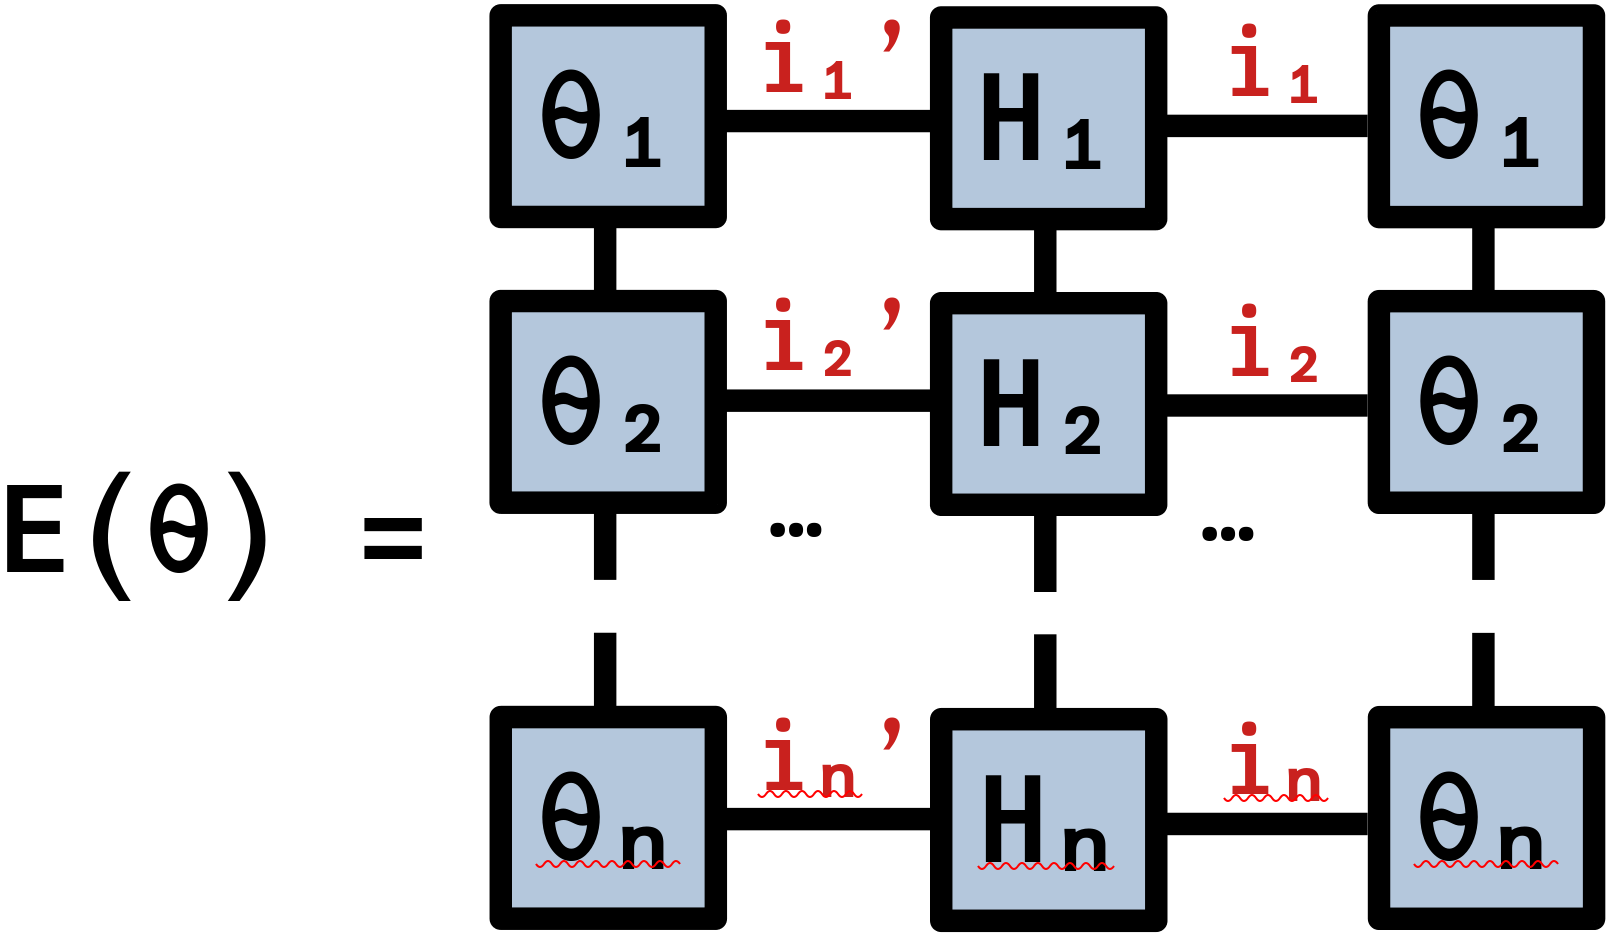
\includegraphics[width=\textwidth]{
  slides/assets/thetan_H_thetan.png
} \\
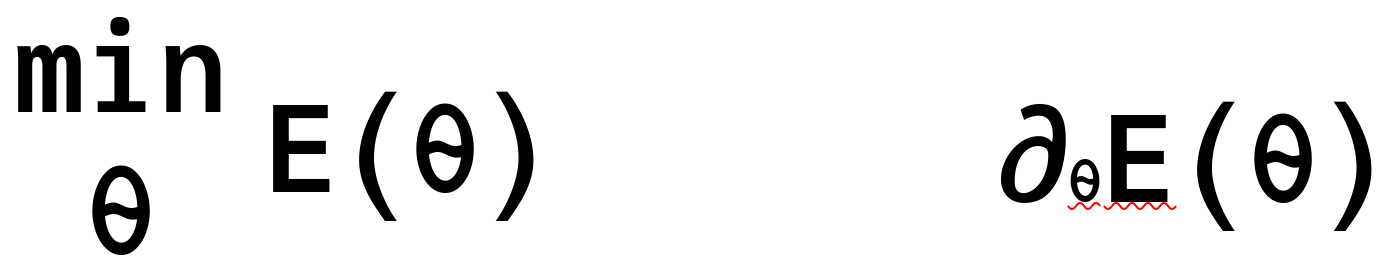
\includegraphics[width=\textwidth]{
  slides/assets/min_grad_E_theta.png
}
\end{center}
\vspace*{0.0cm}
\end{onlyenv}

\end{column}

\end{columns}

\end{frame}
